% Kaplan–Meier estimates of turns survived for the v2 A/B contrast
% (arm A = stock cowrie, arm C = full loop), horizon 30 turns.
% Data: results/field_attack/arm_v2_stats.json (km_a, km_c), written by
% scripts/field_attack_stats_v2.py; both arms censor 16 of 20 sessions
% at their persona-scaled caps.
\begin{figure}[t]
\centering
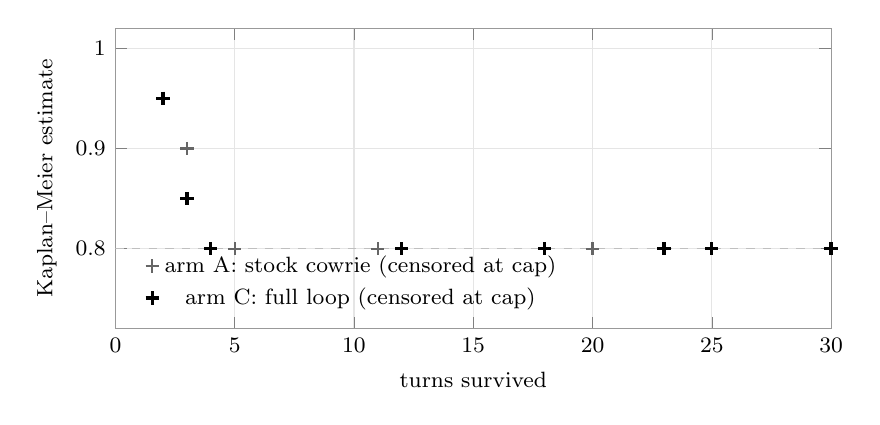
\begin{tikzpicture}
\begin{axis}[
  width=0.88\linewidth,
  height=5.4cm,
  xmin=0, xmax=30,
  ymin=0.72, ymax=1.02,
  xlabel={turns survived},
  ylabel={Kaplan--Meier estimate},
  xlabel style={font=\footnotesize},
  ylabel style={font=\footnotesize},
  tick label style={font=\footnotesize},
  legend style={font=\footnotesize, at={(0.03,0.03)}, anchor=south west, draw=none, fill=none},
  grid=major,
  grid style={black!10},
  axis line style={black!40},
]
% Arm A: stock cowrie
\addplot[
  color=black!60, thick, dash pattern=on 4pt off 2pt,
  mark=+, only marks, mark size=2.4,
  mark options={solid, black!60},
] coordinates {
  (2,0.95) (3,0.90) (4,0.80) (5,0.80) (11,0.80)
  (12,0.80) (18,0.80) (20,0.80) (25,0.80) (30,0.80)
};
\addlegendentry{arm A: stock cowrie (censored at cap)}
% Arm C: full loop
\addplot[
  color=black, very thick,
  mark=+, only marks, mark size=2.4,
  mark options={solid, black},
] coordinates {
  (2,0.95) (3,0.85) (4,0.80) (12,0.80) (18,0.80)
  (23,0.80) (25,0.80) (30,0.80)
};
\addlegendentry{arm C: full loop (censored at cap)}
\addplot[black!25, dashed, thin, domain=0:30] {0.80};
\end{axis}
\end{tikzpicture}
\caption{Kaplan--Meier estimates of turns survived under the v2
pre-registration ($n{=}20$ per arm, horizon 30, persona-scaled caps).
The curves coincide from turn 4 onward: every attacker still engaged at
turn 4 remains to the horizon, and 16 of 20 sessions per arm are censored
at their cap. Saturation, not separation, is the measured outcome
(\texttt{results/field\_attack/arm\_v2\_stats.json}).}
\label{fig:km}
\end{figure}
